% Generated by hw1/scripts/generate_results.py. Do not edit by hand.
Expansion 100 is shown as the baseline. Higher expansion limits are included only when they catch a target missed by the baseline or reduce path cost by at least 5\%.

\subsection*{Map 1}

\subsubsection*{RTAA 100}
\begin{center}
\begin{tabular}{lr}
\textbf{Metric} & \textbf{Value} \\
\hline
Target caught & Yes \\
Time taken (s) & 5316 \\
Total planning time (s) & 10.038632 \\
Moves made & 5027 \\
Path cost & 5316 \\
\end{tabular}
\end{center}
\begin{figure}[H]
  \centering
  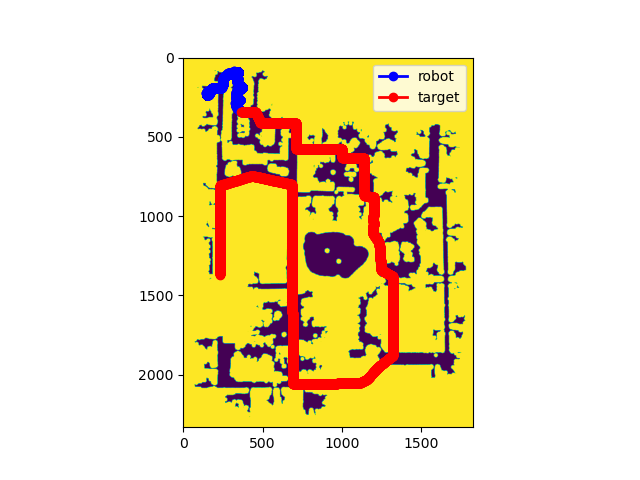
\includegraphics[width=0.92\linewidth]{figures/map1_rtaa_100.png}
  \caption{Final robot and target trajectories for Map 1 using RTAA with expansion limit 100.}
  \label{fig:map1-rtaa-100}
\end{figure}

\subsubsection*{LSS-LRTA 100}
\begin{center}
\begin{tabular}{lr}
\textbf{Metric} & \textbf{Value} \\
\hline
Target caught & Yes \\
Time taken (s) & 5316 \\
Total planning time (s) & 13.109973 \\
Moves made & 5314 \\
Path cost & 5316 \\
\end{tabular}
\end{center}
\begin{figure}[H]
  \centering
  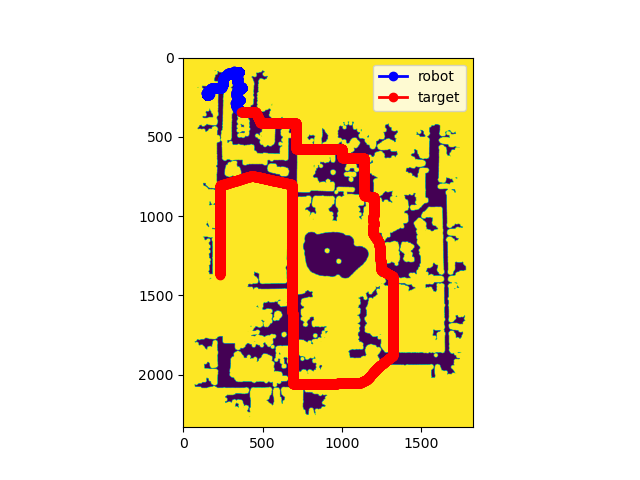
\includegraphics[width=0.92\linewidth]{figures/map1_lss_lrta_100.png}
  \caption{Final robot and target trajectories for Map 1 using LSS-LRTA with expansion limit 100.}
  \label{fig:map1-lss_lrta-100}
\end{figure}

\clearpage

\subsection*{Map 2}

\subsubsection*{RTAA 100}
\begin{center}
\begin{tabular}{lr}
\textbf{Metric} & \textbf{Value} \\
\hline
Target caught & Yes \\
Time taken (s) & 5217 \\
Total planning time (s) & 17.070871 \\
Moves made & 5216 \\
Path cost & 2852354 \\
\end{tabular}
\end{center}
\begin{figure}[H]
  \centering
  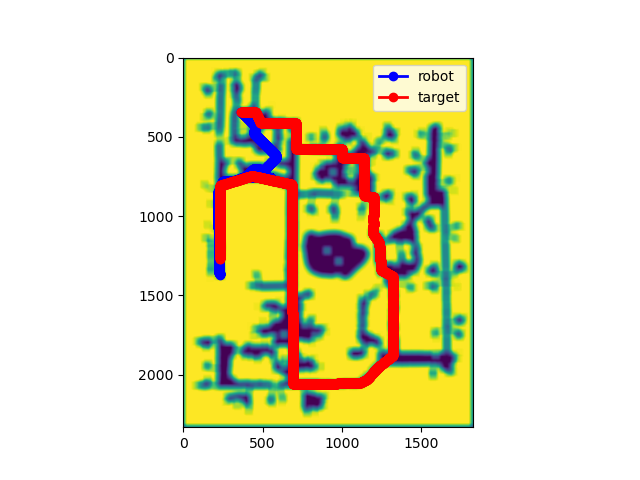
\includegraphics[width=0.92\linewidth]{figures/map2_rtaa_100.png}
  \caption{Final robot and target trajectories for Map 2 using RTAA with expansion limit 100.}
  \label{fig:map2-rtaa-100}
\end{figure}

\subsubsection*{LSS-LRTA 100}
\begin{center}
\begin{tabular}{lr}
\textbf{Metric} & \textbf{Value} \\
\hline
Target caught & Yes \\
Time taken (s) & 5217 \\
Total planning time (s) & 21.782582 \\
Moves made & 5211 \\
Path cost & 2851461 \\
\end{tabular}
\end{center}
\begin{figure}[H]
  \centering
  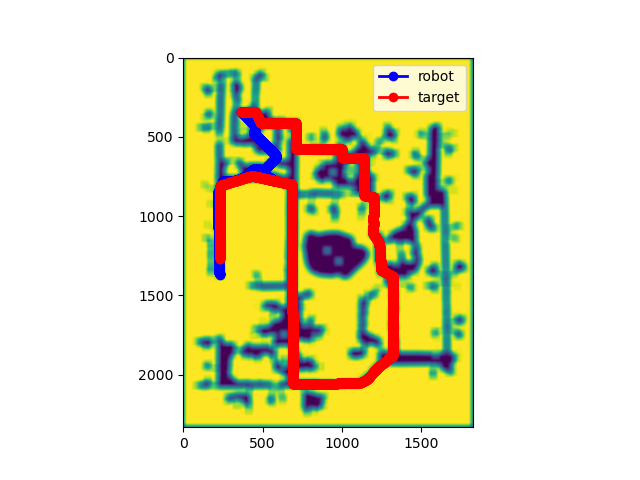
\includegraphics[width=0.92\linewidth]{figures/map2_lss_lrta_100.png}
  \caption{Final robot and target trajectories for Map 2 using LSS-LRTA with expansion limit 100.}
  \label{fig:map2-lss_lrta-100}
\end{figure}

\clearpage

\subsection*{Map 3}

\subsubsection*{RTAA 100}
\begin{center}
\begin{tabular}{lr}
\textbf{Metric} & \textbf{Value} \\
\hline
Target caught & Yes \\
Time taken (s) & 241 \\
Total planning time (s) & 1.141930 \\
Moves made & 241 \\
Path cost & 241 \\
\end{tabular}
\end{center}
\begin{figure}[H]
  \centering
  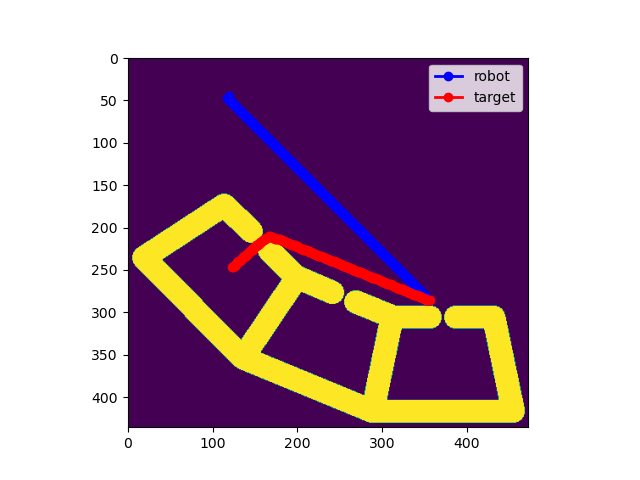
\includegraphics[width=0.92\linewidth]{figures/map3_rtaa_100.png}
  \caption{Final robot and target trajectories for Map 3 using RTAA with expansion limit 100.}
  \label{fig:map3-rtaa-100}
\end{figure}

\subsubsection*{LSS-LRTA 100}
\begin{center}
\begin{tabular}{lr}
\textbf{Metric} & \textbf{Value} \\
\hline
Target caught & Yes \\
Time taken (s) & 241 \\
Total planning time (s) & 1.707082 \\
Moves made & 241 \\
Path cost & 241 \\
\end{tabular}
\end{center}
\begin{figure}[H]
  \centering
  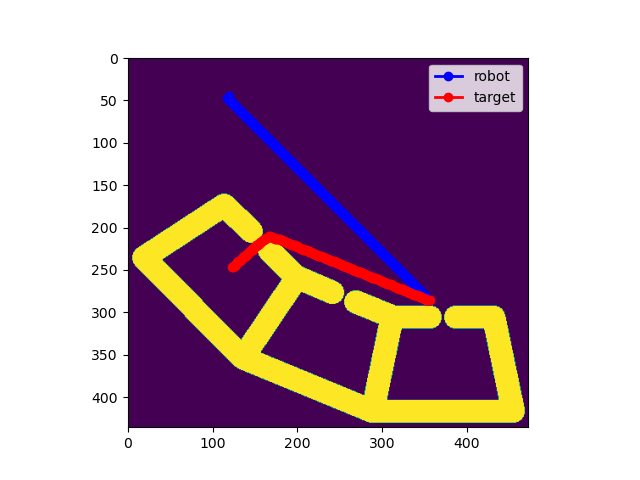
\includegraphics[width=0.92\linewidth]{figures/map3_lss_lrta_100.png}
  \caption{Final robot and target trajectories for Map 3 using LSS-LRTA with expansion limit 100.}
  \label{fig:map3-lss_lrta-100}
\end{figure}

\clearpage

\subsection*{Map 4}

\subsubsection*{RTAA 100}
\begin{center}
\begin{tabular}{lr}
\textbf{Metric} & \textbf{Value} \\
\hline
Target caught & Yes \\
Time taken (s) & 377 \\
Total planning time (s) & 1.334541 \\
Moves made & 377 \\
Path cost & 377 \\
\end{tabular}
\end{center}
\begin{figure}[H]
  \centering
  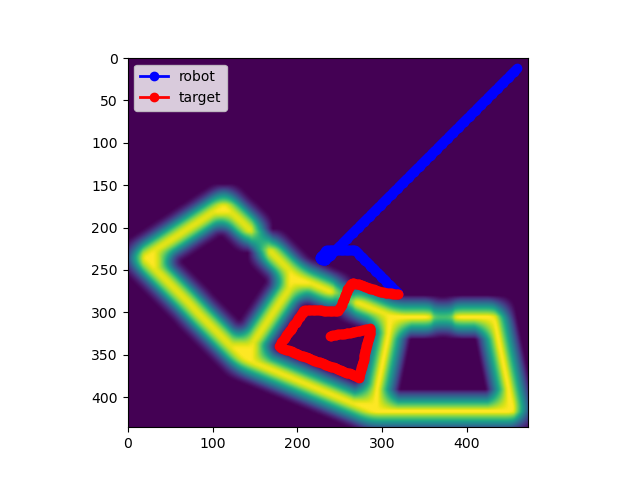
\includegraphics[width=0.92\linewidth]{figures/map4_rtaa_100.png}
  \caption{Final robot and target trajectories for Map 4 using RTAA with expansion limit 100.}
  \label{fig:map4-rtaa-100}
\end{figure}

\subsubsection*{LSS-LRTA 100}
\begin{center}
\begin{tabular}{lr}
\textbf{Metric} & \textbf{Value} \\
\hline
Target caught & Yes \\
Time taken (s) & 377 \\
Total planning time (s) & 1.700465 \\
Moves made & 377 \\
Path cost & 377 \\
\end{tabular}
\end{center}
\begin{figure}[H]
  \centering
  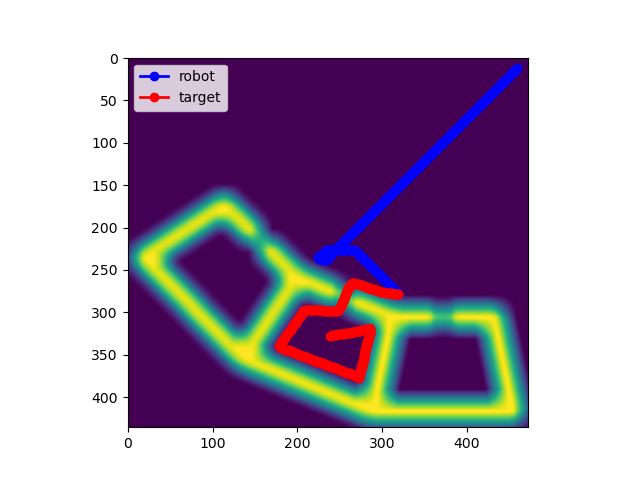
\includegraphics[width=0.92\linewidth]{figures/map4_lss_lrta_100.png}
  \caption{Final robot and target trajectories for Map 4 using LSS-LRTA with expansion limit 100.}
  \label{fig:map4-lss_lrta-100}
\end{figure}

\clearpage

\subsection*{Map 5}

\subsubsection*{RTAA 100}
\begin{center}
\begin{tabular}{lr}
\textbf{Metric} & \textbf{Value} \\
\hline
Target caught & Yes \\
Time taken (s) & 181 \\
Total planning time (s) & 0.314166 \\
Moves made & 181 \\
Path cost & 1357 \\
\end{tabular}
\end{center}
\begin{figure}[H]
  \centering
  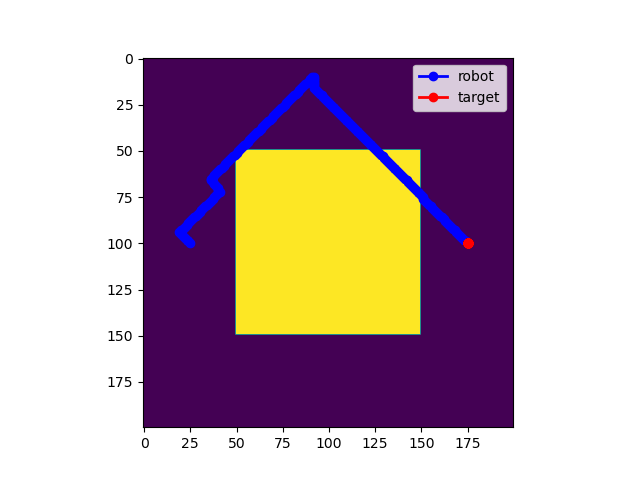
\includegraphics[width=0.92\linewidth]{figures/map5_rtaa_100.png}
  \caption{Final robot and target trajectories for Map 5 using RTAA with expansion limit 100.}
  \label{fig:map5-rtaa-100}
\end{figure}

\subsubsection*{LSS-LRTA 100}
\begin{center}
\begin{tabular}{lr}
\textbf{Metric} & \textbf{Value} \\
\hline
Target caught & Yes \\
Time taken (s) & 181 \\
Total planning time (s) & 0.520379 \\
Moves made & 181 \\
Path cost & 1357 \\
\end{tabular}
\end{center}
\begin{figure}[H]
  \centering
  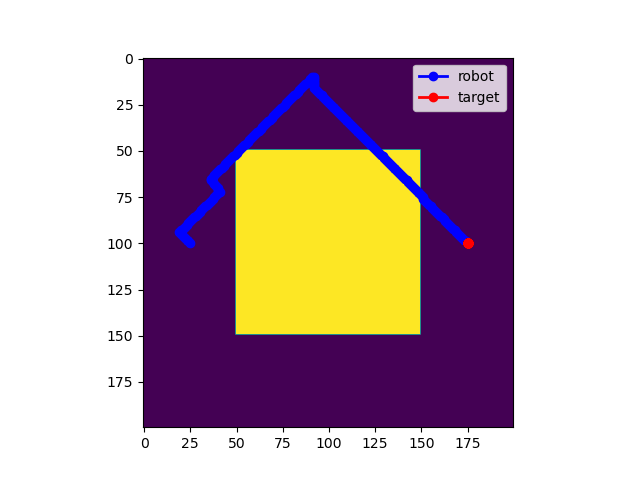
\includegraphics[width=0.92\linewidth]{figures/map5_lss_lrta_100.png}
  \caption{Final robot and target trajectories for Map 5 using LSS-LRTA with expansion limit 100.}
  \label{fig:map5-lss_lrta-100}
\end{figure}

\subsubsection*{RTAA 500}
\begin{center}
\begin{tabular}{lr}
\textbf{Metric} & \textbf{Value} \\
\hline
Target caught & Yes \\
Time taken (s) & 181 \\
Total planning time (s) & 0.718257 \\
Moves made & 181 \\
Path cost & 1210 \\
\end{tabular}
\end{center}
\begin{figure}[H]
  \centering
  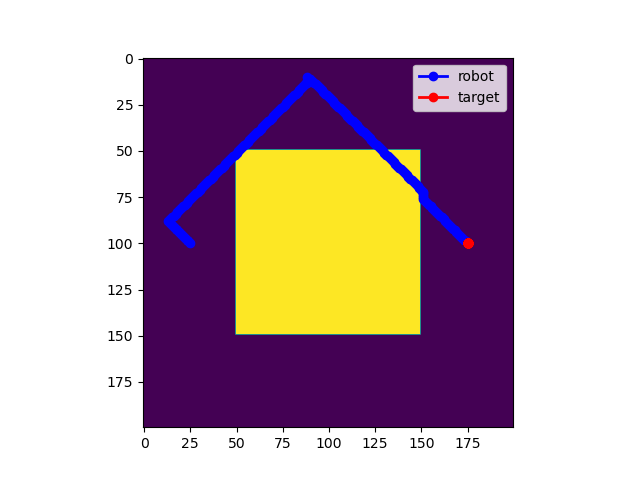
\includegraphics[width=0.92\linewidth]{figures/map5_rtaa_500.png}
  \caption{Final robot and target trajectories for Map 5 using RTAA with expansion limit 500.}
  \label{fig:map5-rtaa-500}
\end{figure}

\subsubsection*{LSS-LRTA 500}
\begin{center}
\begin{tabular}{lr}
\textbf{Metric} & \textbf{Value} \\
\hline
Target caught & Yes \\
Time taken (s) & 181 \\
Total planning time (s) & 1.285368 \\
Moves made & 181 \\
Path cost & 1259 \\
\end{tabular}
\end{center}
\begin{figure}[H]
  \centering
  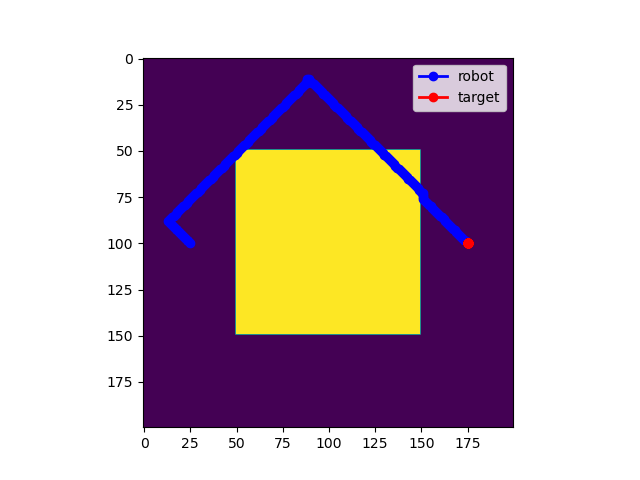
\includegraphics[width=0.92\linewidth]{figures/map5_lss_lrta_500.png}
  \caption{Final robot and target trajectories for Map 5 using LSS-LRTA with expansion limit 500.}
  \label{fig:map5-lss_lrta-500}
\end{figure}

\clearpage

\subsection*{Map 6}

\subsubsection*{RTAA 100}
\begin{center}
\begin{tabular}{lr}
\textbf{Metric} & \textbf{Value} \\
\hline
Target caught & Yes \\
Time taken (s) & 125 \\
Total planning time (s) & 0.283464 \\
Moves made & 125 \\
Path cost & 2500 \\
\end{tabular}
\end{center}
\begin{figure}[H]
  \centering
  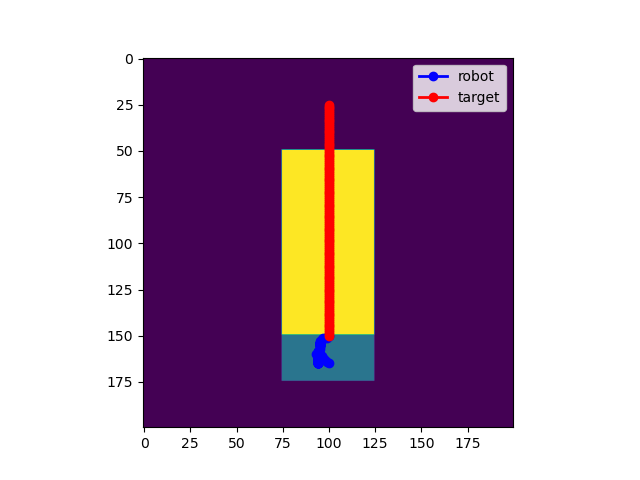
\includegraphics[width=0.92\linewidth]{figures/map6_rtaa_100.png}
  \caption{Final robot and target trajectories for Map 6 using RTAA with expansion limit 100.}
  \label{fig:map6-rtaa-100}
\end{figure}

\subsubsection*{LSS-LRTA 100}
\begin{center}
\begin{tabular}{lr}
\textbf{Metric} & \textbf{Value} \\
\hline
Target caught & Yes \\
Time taken (s) & 125 \\
Total planning time (s) & 0.372342 \\
Moves made & 125 \\
Path cost & 2500 \\
\end{tabular}
\end{center}
\begin{figure}[H]
  \centering
  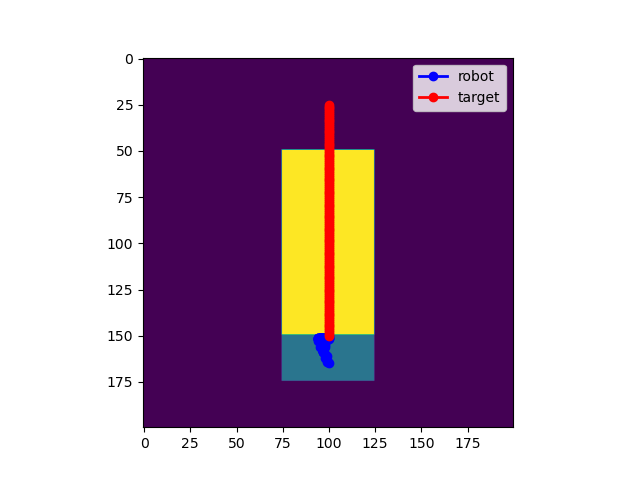
\includegraphics[width=0.92\linewidth]{figures/map6_lss_lrta_100.png}
  \caption{Final robot and target trajectories for Map 6 using LSS-LRTA with expansion limit 100.}
  \label{fig:map6-lss_lrta-100}
\end{figure}

\subsubsection*{RTAA 1000}
\begin{center}
\begin{tabular}{lr}
\textbf{Metric} & \textbf{Value} \\
\hline
Target caught & Yes \\
Time taken (s) & 140 \\
Total planning time (s) & 0.910492 \\
Moves made & 140 \\
Path cost & 843 \\
\end{tabular}
\end{center}
\begin{figure}[H]
  \centering
  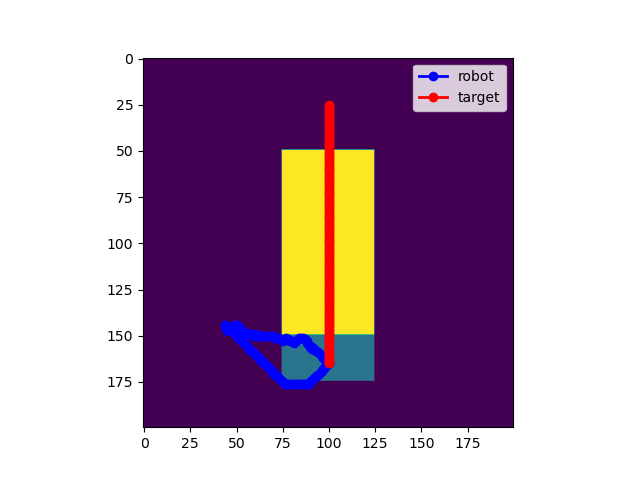
\includegraphics[width=0.92\linewidth]{figures/map6_rtaa_1000.png}
  \caption{Final robot and target trajectories for Map 6 using RTAA with expansion limit 1000.}
  \label{fig:map6-rtaa-1000}
\end{figure}

\subsubsection*{LSS-LRTA 1000}
\begin{center}
\begin{tabular}{lr}
\textbf{Metric} & \textbf{Value} \\
\hline
Target caught & Yes \\
Time taken (s) & 140 \\
Total planning time (s) & 1.466185 \\
Moves made & 140 \\
Path cost & 1014 \\
\end{tabular}
\end{center}
\begin{figure}[H]
  \centering
  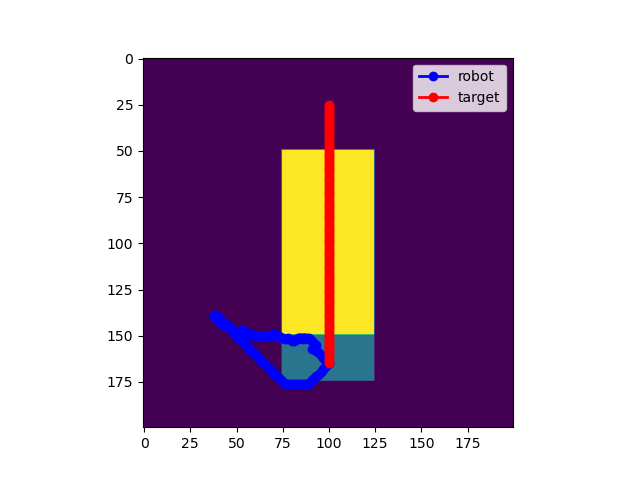
\includegraphics[width=0.92\linewidth]{figures/map6_lss_lrta_1000.png}
  \caption{Final robot and target trajectories for Map 6 using LSS-LRTA with expansion limit 1000.}
  \label{fig:map6-lss_lrta-1000}
\end{figure}

\clearpage

\subsection*{Map 7}

\subsubsection*{RTAA 100}
\begin{center}
\begin{tabular}{lr}
\textbf{Metric} & \textbf{Value} \\
\hline
Target caught & Yes \\
Time taken (s) & 250 \\
Total planning time (s) & 0.966563 \\
Moves made & 250 \\
Path cost & 250 \\
\end{tabular}
\end{center}
\begin{figure}[H]
  \centering
  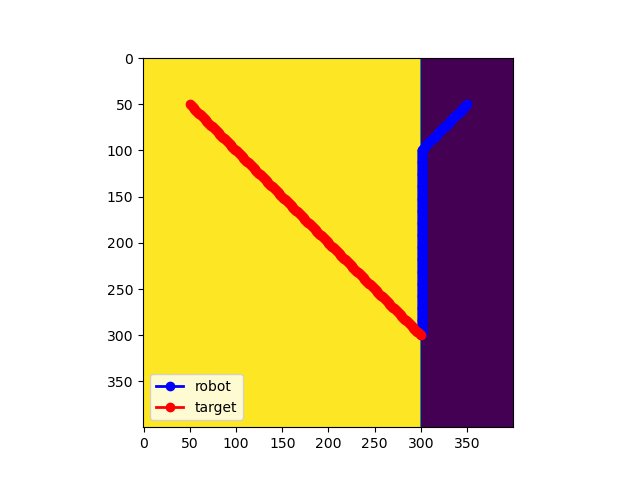
\includegraphics[width=0.92\linewidth]{figures/map7_rtaa_100.png}
  \caption{Final robot and target trajectories for Map 7 using RTAA with expansion limit 100.}
  \label{fig:map7-rtaa-100}
\end{figure}

\subsubsection*{LSS-LRTA 100}
\begin{center}
\begin{tabular}{lr}
\textbf{Metric} & \textbf{Value} \\
\hline
Target caught & Yes \\
Time taken (s) & 250 \\
Total planning time (s) & 1.204509 \\
Moves made & 250 \\
Path cost & 250 \\
\end{tabular}
\end{center}
\begin{figure}[H]
  \centering
  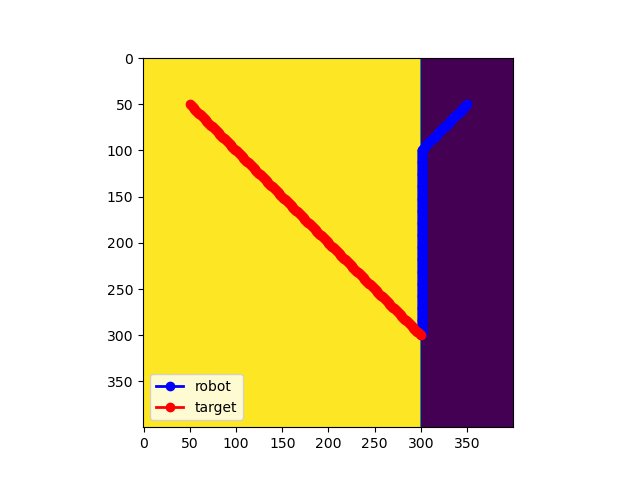
\includegraphics[width=0.92\linewidth]{figures/map7_lss_lrta_100.png}
  \caption{Final robot and target trajectories for Map 7 using LSS-LRTA with expansion limit 100.}
  \label{fig:map7-lss_lrta-100}
\end{figure}

\clearpage

\subsection*{Map 8}

\subsubsection*{RTAA 100}
\begin{center}
\begin{tabular}{lr}
\textbf{Metric} & \textbf{Value} \\
\hline
Target caught & Yes \\
Time taken (s) & 450 \\
Total planning time (s) & 0.901593 \\
Moves made & 450 \\
Path cost & 450 \\
\end{tabular}
\end{center}
\begin{figure}[H]
  \centering
  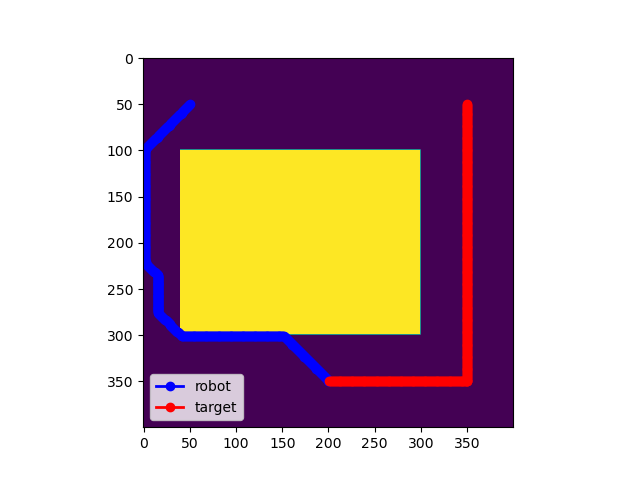
\includegraphics[width=0.92\linewidth]{figures/map8_rtaa_100.png}
  \caption{Final robot and target trajectories for Map 8 using RTAA with expansion limit 100.}
  \label{fig:map8-rtaa-100}
\end{figure}

\subsubsection*{LSS-LRTA 100}
\begin{center}
\begin{tabular}{lr}
\textbf{Metric} & \textbf{Value} \\
\hline
Target caught & Yes \\
Time taken (s) & 450 \\
Total planning time (s) & 1.369250 \\
Moves made & 450 \\
Path cost & 450 \\
\end{tabular}
\end{center}
\begin{figure}[H]
  \centering
  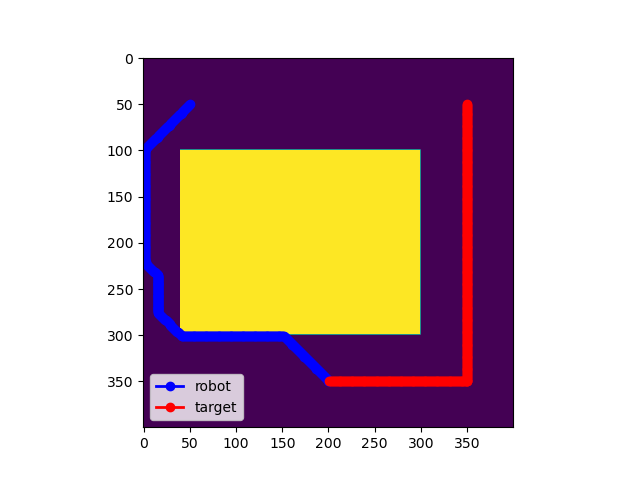
\includegraphics[width=0.92\linewidth]{figures/map8_lss_lrta_100.png}
  \caption{Final robot and target trajectories for Map 8 using LSS-LRTA with expansion limit 100.}
  \label{fig:map8-lss_lrta-100}
\end{figure}

\clearpage

\subsection*{Map 9}

\subsubsection*{RTAA 100}
\begin{center}
\begin{tabular}{lr}
\textbf{Metric} & \textbf{Value} \\
\hline
Target caught & Yes \\
Time taken (s) & 400 \\
Total planning time (s) & 1.130461 \\
Moves made & 400 \\
Path cost & 400 \\
\end{tabular}
\end{center}
\begin{figure}[H]
  \centering
  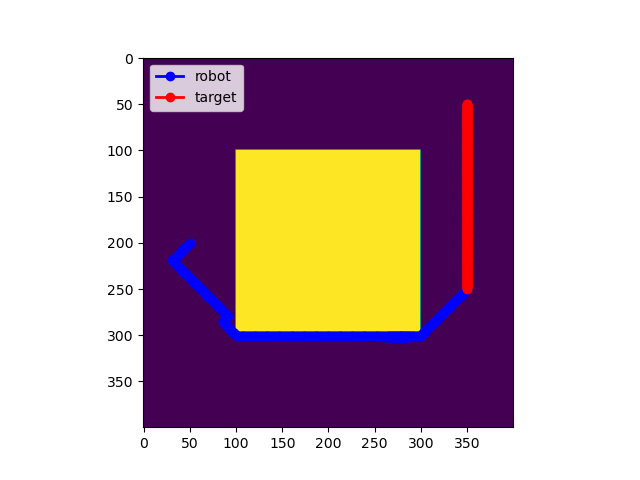
\includegraphics[width=0.92\linewidth]{figures/map9_rtaa_100.png}
  \caption{Final robot and target trajectories for Map 9 using RTAA with expansion limit 100.}
  \label{fig:map9-rtaa-100}
\end{figure}

\subsubsection*{LSS-LRTA 100}
\begin{center}
\begin{tabular}{lr}
\textbf{Metric} & \textbf{Value} \\
\hline
Target caught & Yes \\
Time taken (s) & 400 \\
Total planning time (s) & 2.374034 \\
Moves made & 400 \\
Path cost & 400 \\
\end{tabular}
\end{center}
\begin{figure}[H]
  \centering
  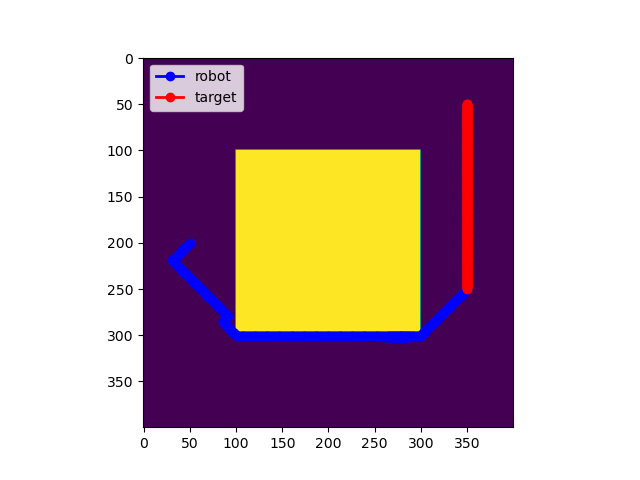
\includegraphics[width=0.92\linewidth]{figures/map9_lss_lrta_100.png}
  \caption{Final robot and target trajectories for Map 9 using LSS-LRTA with expansion limit 100.}
  \label{fig:map9-lss_lrta-100}
\end{figure}

